% Options for packages loaded elsewhere
% Options for packages loaded elsewhere
\PassOptionsToPackage{unicode}{hyperref}
\PassOptionsToPackage{hyphens}{url}
\PassOptionsToPackage{dvipsnames,svgnames,x11names}{xcolor}
%
\documentclass[
  letterpaper,
  DIV=11,
  numbers=noendperiod]{scrartcl}
\usepackage{xcolor}
\usepackage{amsmath,amssymb}
\setcounter{secnumdepth}{-\maxdimen} % remove section numbering
\usepackage{iftex}
\ifPDFTeX
  \usepackage[T1]{fontenc}
  \usepackage[utf8]{inputenc}
  \usepackage{textcomp} % provide euro and other symbols
\else % if luatex or xetex
  \usepackage{unicode-math} % this also loads fontspec
  \defaultfontfeatures{Scale=MatchLowercase}
  \defaultfontfeatures[\rmfamily]{Ligatures=TeX,Scale=1}
\fi
\usepackage{lmodern}
\ifPDFTeX\else
  % xetex/luatex font selection
  \setmainfont[]{TeX Gyre Pagella}
\fi
% Use upquote if available, for straight quotes in verbatim environments
\IfFileExists{upquote.sty}{\usepackage{upquote}}{}
\IfFileExists{microtype.sty}{% use microtype if available
  \usepackage[]{microtype}
  \UseMicrotypeSet[protrusion]{basicmath} % disable protrusion for tt fonts
}{}
\makeatletter
\@ifundefined{KOMAClassName}{% if non-KOMA class
  \IfFileExists{parskip.sty}{%
    \usepackage{parskip}
  }{% else
    \setlength{\parindent}{0pt}
    \setlength{\parskip}{6pt plus 2pt minus 1pt}}
}{% if KOMA class
  \KOMAoptions{parskip=half}}
\makeatother
% Make \paragraph and \subparagraph free-standing
\makeatletter
\ifx\paragraph\undefined\else
  \let\oldparagraph\paragraph
  \renewcommand{\paragraph}{
    \@ifstar
      \xxxParagraphStar
      \xxxParagraphNoStar
  }
  \newcommand{\xxxParagraphStar}[1]{\oldparagraph*{#1}\mbox{}}
  \newcommand{\xxxParagraphNoStar}[1]{\oldparagraph{#1}\mbox{}}
\fi
\ifx\subparagraph\undefined\else
  \let\oldsubparagraph\subparagraph
  \renewcommand{\subparagraph}{
    \@ifstar
      \xxxSubParagraphStar
      \xxxSubParagraphNoStar
  }
  \newcommand{\xxxSubParagraphStar}[1]{\oldsubparagraph*{#1}\mbox{}}
  \newcommand{\xxxSubParagraphNoStar}[1]{\oldsubparagraph{#1}\mbox{}}
\fi
\makeatother

\usepackage{color}
\usepackage{fancyvrb}
\newcommand{\VerbBar}{|}
\newcommand{\VERB}{\Verb[commandchars=\\\{\}]}
\DefineVerbatimEnvironment{Highlighting}{Verbatim}{commandchars=\\\{\}}
% Add ',fontsize=\small' for more characters per line
\usepackage{framed}
\definecolor{shadecolor}{RGB}{241,243,245}
\newenvironment{Shaded}{\begin{snugshade}}{\end{snugshade}}
\newcommand{\AlertTok}[1]{\textcolor[rgb]{0.68,0.00,0.00}{#1}}
\newcommand{\AnnotationTok}[1]{\textcolor[rgb]{0.37,0.37,0.37}{#1}}
\newcommand{\AttributeTok}[1]{\textcolor[rgb]{0.40,0.45,0.13}{#1}}
\newcommand{\BaseNTok}[1]{\textcolor[rgb]{0.68,0.00,0.00}{#1}}
\newcommand{\BuiltInTok}[1]{\textcolor[rgb]{0.00,0.23,0.31}{#1}}
\newcommand{\CharTok}[1]{\textcolor[rgb]{0.13,0.47,0.30}{#1}}
\newcommand{\CommentTok}[1]{\textcolor[rgb]{0.37,0.37,0.37}{#1}}
\newcommand{\CommentVarTok}[1]{\textcolor[rgb]{0.37,0.37,0.37}{\textit{#1}}}
\newcommand{\ConstantTok}[1]{\textcolor[rgb]{0.56,0.35,0.01}{#1}}
\newcommand{\ControlFlowTok}[1]{\textcolor[rgb]{0.00,0.23,0.31}{\textbf{#1}}}
\newcommand{\DataTypeTok}[1]{\textcolor[rgb]{0.68,0.00,0.00}{#1}}
\newcommand{\DecValTok}[1]{\textcolor[rgb]{0.68,0.00,0.00}{#1}}
\newcommand{\DocumentationTok}[1]{\textcolor[rgb]{0.37,0.37,0.37}{\textit{#1}}}
\newcommand{\ErrorTok}[1]{\textcolor[rgb]{0.68,0.00,0.00}{#1}}
\newcommand{\ExtensionTok}[1]{\textcolor[rgb]{0.00,0.23,0.31}{#1}}
\newcommand{\FloatTok}[1]{\textcolor[rgb]{0.68,0.00,0.00}{#1}}
\newcommand{\FunctionTok}[1]{\textcolor[rgb]{0.28,0.35,0.67}{#1}}
\newcommand{\ImportTok}[1]{\textcolor[rgb]{0.00,0.46,0.62}{#1}}
\newcommand{\InformationTok}[1]{\textcolor[rgb]{0.37,0.37,0.37}{#1}}
\newcommand{\KeywordTok}[1]{\textcolor[rgb]{0.00,0.23,0.31}{\textbf{#1}}}
\newcommand{\NormalTok}[1]{\textcolor[rgb]{0.00,0.23,0.31}{#1}}
\newcommand{\OperatorTok}[1]{\textcolor[rgb]{0.37,0.37,0.37}{#1}}
\newcommand{\OtherTok}[1]{\textcolor[rgb]{0.00,0.23,0.31}{#1}}
\newcommand{\PreprocessorTok}[1]{\textcolor[rgb]{0.68,0.00,0.00}{#1}}
\newcommand{\RegionMarkerTok}[1]{\textcolor[rgb]{0.00,0.23,0.31}{#1}}
\newcommand{\SpecialCharTok}[1]{\textcolor[rgb]{0.37,0.37,0.37}{#1}}
\newcommand{\SpecialStringTok}[1]{\textcolor[rgb]{0.13,0.47,0.30}{#1}}
\newcommand{\StringTok}[1]{\textcolor[rgb]{0.13,0.47,0.30}{#1}}
\newcommand{\VariableTok}[1]{\textcolor[rgb]{0.07,0.07,0.07}{#1}}
\newcommand{\VerbatimStringTok}[1]{\textcolor[rgb]{0.13,0.47,0.30}{#1}}
\newcommand{\WarningTok}[1]{\textcolor[rgb]{0.37,0.37,0.37}{\textit{#1}}}

\usepackage{longtable,booktabs,array}
\usepackage{calc} % for calculating minipage widths
% Correct order of tables after \paragraph or \subparagraph
\usepackage{etoolbox}
\makeatletter
\patchcmd\longtable{\par}{\if@noskipsec\mbox{}\fi\par}{}{}
\makeatother
% Allow footnotes in longtable head/foot
\IfFileExists{footnotehyper.sty}{\usepackage{footnotehyper}}{\usepackage{footnote}}
\makesavenoteenv{longtable}
\usepackage{graphicx}
\makeatletter
\newsavebox\pandoc@box
\newcommand*\pandocbounded[1]{% scales image to fit in text height/width
  \sbox\pandoc@box{#1}%
  \Gscale@div\@tempa{\textheight}{\dimexpr\ht\pandoc@box+\dp\pandoc@box\relax}%
  \Gscale@div\@tempb{\linewidth}{\wd\pandoc@box}%
  \ifdim\@tempb\p@<\@tempa\p@\let\@tempa\@tempb\fi% select the smaller of both
  \ifdim\@tempa\p@<\p@\scalebox{\@tempa}{\usebox\pandoc@box}%
  \else\usebox{\pandoc@box}%
  \fi%
}
% Set default figure placement to htbp
\def\fps@figure{htbp}
\makeatother





\setlength{\emergencystretch}{3em} % prevent overfull lines

\providecommand{\tightlist}{%
  \setlength{\itemsep}{0pt}\setlength{\parskip}{0pt}}



 


\KOMAoption{captions}{tableheading}
\makeatletter
\@ifpackageloaded{caption}{}{\usepackage{caption}}
\AtBeginDocument{%
\ifdefined\contentsname
  \renewcommand*\contentsname{Table of contents}
\else
  \newcommand\contentsname{Table of contents}
\fi
\ifdefined\listfigurename
  \renewcommand*\listfigurename{List of Figures}
\else
  \newcommand\listfigurename{List of Figures}
\fi
\ifdefined\listtablename
  \renewcommand*\listtablename{List of Tables}
\else
  \newcommand\listtablename{List of Tables}
\fi
\ifdefined\figurename
  \renewcommand*\figurename{Figure}
\else
  \newcommand\figurename{Figure}
\fi
\ifdefined\tablename
  \renewcommand*\tablename{Table}
\else
  \newcommand\tablename{Table}
\fi
}
\@ifpackageloaded{float}{}{\usepackage{float}}
\floatstyle{ruled}
\@ifundefined{c@chapter}{\newfloat{codelisting}{h}{lop}}{\newfloat{codelisting}{h}{lop}[chapter]}
\floatname{codelisting}{Listing}
\newcommand*\listoflistings{\listof{codelisting}{List of Listings}}
\makeatother
\makeatletter
\makeatother
\makeatletter
\@ifpackageloaded{caption}{}{\usepackage{caption}}
\@ifpackageloaded{subcaption}{}{\usepackage{subcaption}}
\makeatother
\usepackage{bookmark}
\IfFileExists{xurl.sty}{\usepackage{xurl}}{} % add URL line breaks if available
\urlstyle{same}
\hypersetup{
  pdftitle={PS 1},
  pdfauthor={David Cai, Miriam Gold, Ella Moxley, Geoffrey Yip},
  colorlinks=true,
  linkcolor={blue},
  filecolor={Maroon},
  citecolor={Blue},
  urlcolor={Blue},
  pdfcreator={LaTeX via pandoc}}


\title{PS 1}
\usepackage{etoolbox}
\makeatletter
\providecommand{\subtitle}[1]{% add subtitle to \maketitle
  \apptocmd{\@title}{\par {\large #1 \par}}{}{}
}
\makeatother
\subtitle{ARE 212, Spring 2026}
\author{David Cai, Miriam Gold, Ella Moxley, Geoffrey Yip}
\date{2026-02-25}
\begin{document}
\maketitle


\section{Set-up}\label{set-up}

\begin{Shaded}
\begin{Highlighting}[]
\FunctionTok{library}\NormalTok{(WDI)}
\FunctionTok{library}\NormalTok{(tidyverse)}
\end{Highlighting}
\end{Shaded}

\begin{verbatim}
-- Attaching core tidyverse packages ------------------------ tidyverse 2.0.0 --
v dplyr     1.1.4     v readr     2.1.5
v forcats   1.0.0     v stringr   1.5.1
v ggplot2   3.5.2     v tibble    3.2.1
v lubridate 1.9.4     v tidyr     1.3.1
v purrr     1.0.4     
-- Conflicts ------------------------------------------ tidyverse_conflicts() --
x dplyr::filter() masks stats::filter()
x dplyr::lag()    masks stats::lag()
i Use the conflicted package (<http://conflicted.r-lib.org/>) to force all conflicts to become errors
\end{verbatim}

\begin{Shaded}
\begin{Highlighting}[]
\FunctionTok{library}\NormalTok{(magrittr)}
\end{Highlighting}
\end{Shaded}

\begin{verbatim}

Attaching package: 'magrittr'

The following object is masked from 'package:purrr':

    set_names

The following object is masked from 'package:tidyr':

    extract
\end{verbatim}

\begin{Shaded}
\begin{Highlighting}[]
\FunctionTok{library}\NormalTok{(fs)}
\FunctionTok{library}\NormalTok{(janitor)}
\end{Highlighting}
\end{Shaded}

\begin{verbatim}

Attaching package: 'janitor'

The following objects are masked from 'package:stats':

    chisq.test, fisher.test
\end{verbatim}

\begin{Shaded}
\begin{Highlighting}[]
\CommentTok{\# Paths ==================}
\NormalTok{path }\OtherTok{\textless{}{-}} \StringTok{"/Users/miriamgold/projects/ARE212\_2026/ps1"}
\NormalTok{path\_functions }\OtherTok{\textless{}{-}} \FunctionTok{file.path}\NormalTok{(path, }\StringTok{"functions"}\NormalTok{)}
\NormalTok{path\_data }\OtherTok{\textless{}{-}} \FunctionTok{file.path}\NormalTok{(path, }\StringTok{"data"}\NormalTok{)}

\CommentTok{\# Source custom functions }
\FunctionTok{dir\_walk}\NormalTok{(path\_functions, source)}

\CommentTok{\# Data setup ==============}

\NormalTok{iso\_codes }\OtherTok{\textless{}{-}} 
  \FunctionTok{read\_csv}\NormalTok{(}\StringTok{"https://gist.githubusercontent.com/radcliff/f09c0f88344a7fcef373/raw/2753c482ad091c54b1822288ad2e4811c021d8ec/wikipedia{-}iso{-}country{-}codes.csv"}\NormalTok{)}
\end{Highlighting}
\end{Shaded}

\begin{verbatim}
Rows: 246 Columns: 5
-- Column specification --------------------------------------------------------
Delimiter: ","
chr (5): English short name lower case, Alpha-2 code, Alpha-3 code, Numeric ...

i Use `spec()` to retrieve the full column specification for this data.
i Specify the column types or set `show_col_types = FALSE` to quiet this message.
\end{verbatim}

\begin{Shaded}
\begin{Highlighting}[]
\NormalTok{wb\_vars }\OtherTok{\textless{}{-}} \FunctionTok{c}\NormalTok{(}\StringTok{"EN.GHG.CO2.MT.CE.AR5"}\NormalTok{, }\StringTok{"NY.GDP.MKTP.KD"}\NormalTok{, }\StringTok{"SP.POP.TOTL"}\NormalTok{)}

\NormalTok{wdi\_avail\_countries }\OtherTok{\textless{}{-}} 
\NormalTok{  WDI}\SpecialCharTok{::}\NormalTok{WDI\_data }\SpecialCharTok{\%\textgreater{}\%}
\NormalTok{  purrr}\SpecialCharTok{::}\FunctionTok{pluck}\NormalTok{(}\DecValTok{2}\NormalTok{) }\SpecialCharTok{\%\textgreater{}\%} 
  \FunctionTok{pull}\NormalTok{(iso2c)}

\NormalTok{countries }\OtherTok{\textless{}{-}} 
\NormalTok{  iso\_codes }\SpecialCharTok{|\textgreater{}}
  \FunctionTok{filter}\NormalTok{(}\StringTok{\textasciigrave{}}\AttributeTok{Alpha{-}2 code}\StringTok{\textasciigrave{}} \SpecialCharTok{\%in\%}\NormalTok{ wdi\_avail\_countries) }\SpecialCharTok{\%\textgreater{}\%}
  \FunctionTok{pull}\NormalTok{(}\StringTok{"Alpha{-}2 code"}\NormalTok{)}
\end{Highlighting}
\end{Shaded}

\section{Q1}\label{q1}

\begin{Shaded}
\begin{Highlighting}[]
\CommentTok{\# I had to disable the automatic data fetching because the WB API servers stopped responding}
\ControlFlowTok{if}\NormalTok{(}\ConstantTok{FALSE}\NormalTok{)\{}
\NormalTok{wdi\_data\_raw }\OtherTok{\textless{}{-}} 
\NormalTok{  countries }\SpecialCharTok{\%\textgreater{}\%}
\NormalTok{  purrr}\SpecialCharTok{::}\FunctionTok{map}\NormalTok{(}\SpecialCharTok{\textasciitilde{}}\FunctionTok{wdi\_noisy}\NormalTok{(}\AttributeTok{country =}\NormalTok{ .x, }\AttributeTok{indicator=}\NormalTok{wb\_vars, }\AttributeTok{start=}\DecValTok{2010}\NormalTok{, }\AttributeTok{end=}\DecValTok{2010}\NormalTok{)) }\SpecialCharTok{\%\textgreater{}\%}
\NormalTok{  purrr}\SpecialCharTok{::}\FunctionTok{list\_rbind}\NormalTok{()}
\NormalTok{\}}

\NormalTok{wdi\_data\_raw }\OtherTok{\textless{}{-}}
  \FunctionTok{read\_csv}\NormalTok{(}
    \FunctionTok{file.path}\NormalTok{(path\_data, }\StringTok{"48038096{-}3fbd{-}47af{-}8962{-}7f774cfef8a8\_Data.csv"}\NormalTok{)}
\NormalTok{  )}
\end{Highlighting}
\end{Shaded}

\begin{verbatim}
Rows: 656 Columns: 5
-- Column specification --------------------------------------------------------
Delimiter: ","
chr (5): Country Name, Country Code, Series Name, Series Code, 2010 [YR2010]

i Use `spec()` to retrieve the full column specification for this data.
i Specify the column types or set `show_col_types = FALSE` to quiet this message.
\end{verbatim}

\section{Q2}\label{q2}

\begin{Shaded}
\begin{Highlighting}[]
\NormalTok{wdi\_data\_clean }\OtherTok{\textless{}{-}} 
\NormalTok{  wdi\_data\_raw }\SpecialCharTok{|\textgreater{}}
  \FunctionTok{clean\_names}\NormalTok{() }\SpecialCharTok{\%\textgreater{}\%}
  \FunctionTok{drop\_na}\NormalTok{() }\SpecialCharTok{\%\textgreater{}\%}
  \FunctionTok{select}\NormalTok{(country\_code, series\_code, x2010\_yr2010) }\SpecialCharTok{\%\textgreater{}\%}
  \FunctionTok{mutate}\NormalTok{(}
    \AttributeTok{var\_name =} \FunctionTok{case\_when}\NormalTok{(}
\NormalTok{      series\_code }\SpecialCharTok{==} \StringTok{"EN.GHG.CO2.MT.CE.AR5"} \SpecialCharTok{\textasciitilde{}} \StringTok{"CO2"}\NormalTok{,}
\NormalTok{      series\_code }\SpecialCharTok{==} \StringTok{"NY.GDP.MKTP.KD"} \SpecialCharTok{\textasciitilde{}} \StringTok{"GDP"}\NormalTok{,}
\NormalTok{      series\_code }\SpecialCharTok{==} \StringTok{"SP.POP.TOTL"} \SpecialCharTok{\textasciitilde{}} \StringTok{"POP"}
\NormalTok{    ),}
    \AttributeTok{x2010\_yr2010 =} \FunctionTok{as.numeric}\NormalTok{(x2010\_yr2010)}
\NormalTok{  ) }\SpecialCharTok{|\textgreater{}}
    \FunctionTok{rename}\NormalTok{(}\AttributeTok{country =}\NormalTok{ country\_code) }\SpecialCharTok{\%\textgreater{}\%}
    \FunctionTok{pivot\_wider}\NormalTok{(}
      \AttributeTok{id\_cols =}\NormalTok{ country,}
      \AttributeTok{names\_from =} \StringTok{"var\_name"}\NormalTok{,}
      \AttributeTok{values\_from =} \StringTok{"x2010\_yr2010"}
\NormalTok{    ) }\SpecialCharTok{\%\textgreater{}\%}
  \FunctionTok{drop\_na}\NormalTok{()}
\end{Highlighting}
\end{Shaded}

\begin{verbatim}
Warning: There was 1 warning in `mutate()`.
i In argument: `x2010_yr2010 = as.numeric(x2010_yr2010)`.
Caused by warning:
! NAs introduced by coercion
\end{verbatim}

\section{Q3}\label{q3}

\begin{Shaded}
\begin{Highlighting}[]
\NormalTok{wdi\_summary\_stats }\OtherTok{\textless{}{-}} 
\NormalTok{  wdi\_data\_clean }\SpecialCharTok{|\textgreater{}}
   \FunctionTok{pivot\_longer}\NormalTok{(}\AttributeTok{cols =} \FunctionTok{c}\NormalTok{(}\StringTok{"CO2"}\NormalTok{, }\StringTok{"GDP"}\NormalTok{, }\StringTok{"POP"}\NormalTok{), }\AttributeTok{names\_to =} \StringTok{"var"}\NormalTok{) }\SpecialCharTok{|\textgreater{}}
   \FunctionTok{group\_by}\NormalTok{(var) }\SpecialCharTok{|\textgreater{}}
   \FunctionTok{summarise}\NormalTok{(}
    \AttributeTok{mean =} \FunctionTok{mean}\NormalTok{(value),}
    \AttributeTok{sd =} \FunctionTok{sd}\NormalTok{(value),}
    \AttributeTok{min =} \FunctionTok{min}\NormalTok{(value),}
    \AttributeTok{max =} \FunctionTok{max}\NormalTok{(value)}
\NormalTok{   )}
\FunctionTok{print}\NormalTok{(wdi\_summary\_stats)}
\end{Highlighting}
\end{Shaded}

\begin{verbatim}
# A tibble: 3 x 5
  var            mean      sd       min     max
  <chr>         <dbl>   <dbl>     <dbl>   <dbl>
1 CO2            164. 7.81e 2        0  9.11e 3
2 GDP   325737923786. 1.36e12 30560853. 1.63e13
3 POP       34989968. 1.34e 8    10043  1.34e 9
\end{verbatim}

\section{Q4}\label{q4}

\begin{Shaded}
\begin{Highlighting}[]
\NormalTok{wdi\_data\_clean }\SpecialCharTok{\%\textgreater{}\%}
   \FunctionTok{pivot\_longer}\NormalTok{(}\AttributeTok{cols =} \FunctionTok{c}\NormalTok{(}\StringTok{"CO2"}\NormalTok{, }\StringTok{"GDP"}\NormalTok{, }\StringTok{"POP"}\NormalTok{), }\AttributeTok{names\_to =} \StringTok{"var"}\NormalTok{) }\SpecialCharTok{\%\textgreater{}\%}
  \FunctionTok{filter}\NormalTok{(var }\SpecialCharTok{\%in\%} \FunctionTok{c}\NormalTok{(}\StringTok{"CO2"}\NormalTok{, }\StringTok{"GDP"}\NormalTok{)) }\SpecialCharTok{\%\textgreater{}\%}
  \FunctionTok{ggplot}\NormalTok{(}\FunctionTok{aes}\NormalTok{(}\AttributeTok{x =}\NormalTok{ value, }\AttributeTok{fill =}\NormalTok{ var)) }\SpecialCharTok{+}
  \FunctionTok{geom\_histogram}\NormalTok{(}\AttributeTok{bins =} \DecValTok{15}\NormalTok{, }\AttributeTok{position =} \StringTok{"dodge"}\NormalTok{) }\SpecialCharTok{+}
  \FunctionTok{scale\_fill\_discrete}\NormalTok{(}\AttributeTok{name =} \ConstantTok{NULL}\NormalTok{) }\SpecialCharTok{+}
  \FunctionTok{theme\_bw}\NormalTok{()}
\end{Highlighting}
\end{Shaded}

\pandocbounded{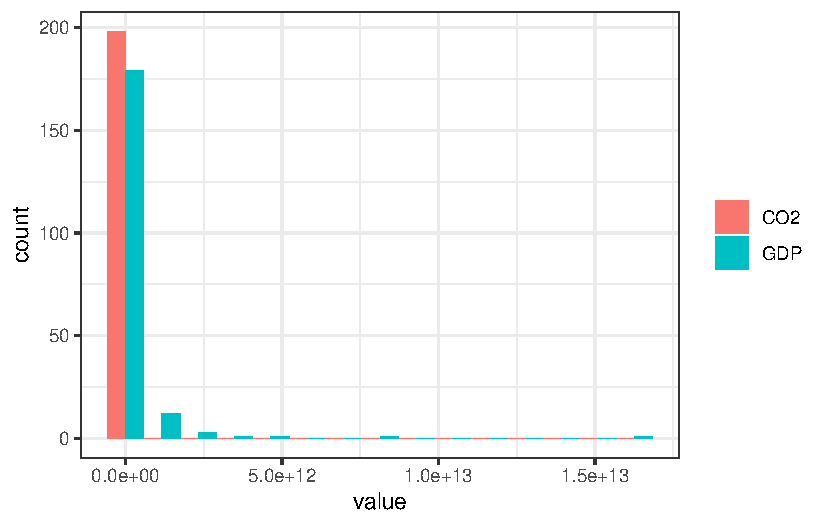
\includegraphics[keepaspectratio]{are212_ps1_files/figure-pdf/unnamed-chunk-5-1.pdf}}

\section{Q5}\label{q5}

\begin{Shaded}
\begin{Highlighting}[]
\NormalTok{wdi\_data\_clean }\SpecialCharTok{\%\textgreater{}\%}
  \FunctionTok{ggplot}\NormalTok{(}\FunctionTok{aes}\NormalTok{(}\AttributeTok{x =}\NormalTok{ GDP, }\AttributeTok{y =}\NormalTok{ CO2)) }\SpecialCharTok{+}
  \FunctionTok{geom\_point}\NormalTok{() }\SpecialCharTok{+}
  \FunctionTok{scale\_x\_continuous}\NormalTok{(}\StringTok{"Gross Domestic Product (constant USD)"}\NormalTok{) }\SpecialCharTok{+}
  \FunctionTok{scale\_y\_continuous}\NormalTok{(}\StringTok{"CO2 Emissions (mt)"}\NormalTok{) }\SpecialCharTok{+}
  \FunctionTok{labs}\NormalTok{(}
    \AttributeTok{title =} \StringTok{"Country{-}level Carbon Emissions against GDP (2010)"}
\NormalTok{  ) }\SpecialCharTok{+}
  \FunctionTok{theme\_bw}\NormalTok{()}
\end{Highlighting}
\end{Shaded}

\pandocbounded{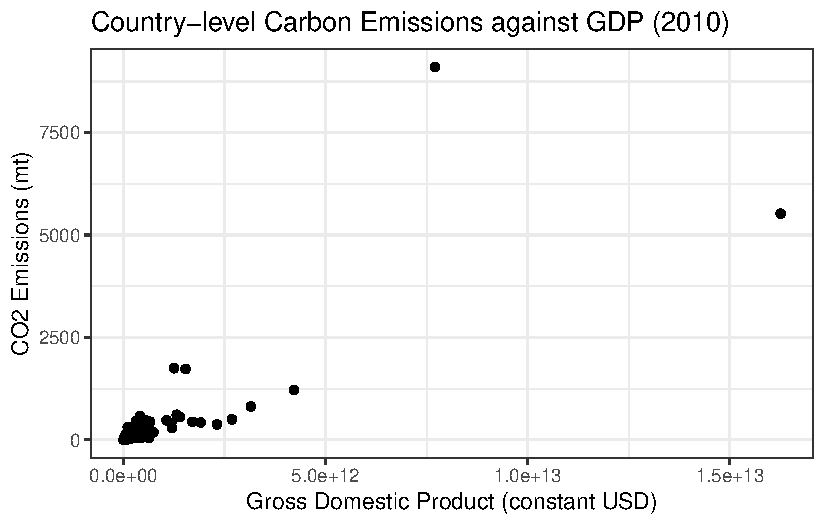
\includegraphics[keepaspectratio]{are212_ps1_files/figure-pdf/unnamed-chunk-6-1.pdf}}

\section{Q6/7}\label{q67}

\begin{Shaded}
\begin{Highlighting}[]
\NormalTok{wdi\_per\_capita }\OtherTok{\textless{}{-}}
\NormalTok{  wdi\_data\_clean }\SpecialCharTok{\%\textgreater{}\%}
  \FunctionTok{mutate}\NormalTok{(}
    \AttributeTok{CO2pc =}\NormalTok{ CO2}\SpecialCharTok{/}\NormalTok{POP,}
    \AttributeTok{GDPpc =}\NormalTok{ GDP}\SpecialCharTok{/}\NormalTok{POP}
\NormalTok{  )}
\end{Highlighting}
\end{Shaded}

\section{Q8}\label{q8}

\begin{Shaded}
\begin{Highlighting}[]
\NormalTok{wdi\_per\_capita }\SpecialCharTok{\%\textgreater{}\%}
  \FunctionTok{ggplot}\NormalTok{(}\FunctionTok{aes}\NormalTok{(}\AttributeTok{x =}\NormalTok{ GDPpc, }\AttributeTok{y =}\NormalTok{ CO2pc)) }\SpecialCharTok{+}
  \FunctionTok{geom\_point}\NormalTok{() }\SpecialCharTok{+}
  \FunctionTok{scale\_x\_continuous}\NormalTok{(}\StringTok{"GDP (constant USD/capita)"}\NormalTok{) }\SpecialCharTok{+}
  \FunctionTok{scale\_y\_continuous}\NormalTok{(}\StringTok{"CO2 Emissions (mt/capita)"}\NormalTok{) }\SpecialCharTok{+}
  \FunctionTok{labs}\NormalTok{(}
    \AttributeTok{title =} \StringTok{"Per capita carbon emissions and GDP (2010)"}
\NormalTok{  ) }\SpecialCharTok{+}
  \FunctionTok{theme\_bw}\NormalTok{()}
\end{Highlighting}
\end{Shaded}

\pandocbounded{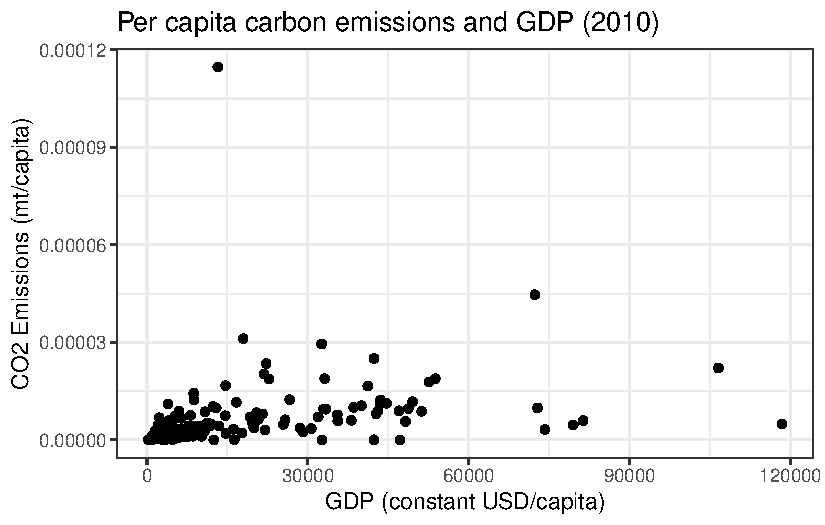
\includegraphics[keepaspectratio]{are212_ps1_files/figure-pdf/unnamed-chunk-8-1.pdf}}

\section{Q9}\label{q9}

\begin{Shaded}
\begin{Highlighting}[]
\NormalTok{wdi\_per\_capita\_demeaned }\OtherTok{\textless{}{-}} 
\NormalTok{  wdi\_per\_capita }\SpecialCharTok{\%\textgreater{}\%}
  \FunctionTok{mutate}\NormalTok{(}
    \AttributeTok{CO2pcdev =}\NormalTok{ CO2pc}\SpecialCharTok{{-}}\FunctionTok{mean}\NormalTok{(CO2pc),}
    \AttributeTok{GDPpcdev =}\NormalTok{ GDPpc}\SpecialCharTok{{-}}\FunctionTok{mean}\NormalTok{(GDPpc)}
\NormalTok{  )}
\end{Highlighting}
\end{Shaded}

\section{Q10}\label{q10}

\begin{Shaded}
\begin{Highlighting}[]
\NormalTok{wdi\_per\_capita\_demeaned }\SpecialCharTok{\%\textgreater{}\%}
  \FunctionTok{ggplot}\NormalTok{(}\FunctionTok{aes}\NormalTok{(}\AttributeTok{x =}\NormalTok{ GDPpcdev, }\AttributeTok{y =}\NormalTok{ CO2pcdev)) }\SpecialCharTok{+}
  \FunctionTok{geom\_point}\NormalTok{() }\SpecialCharTok{+}
  \FunctionTok{scale\_x\_continuous}\NormalTok{(}\StringTok{"Demeaned GDP (constant USD/capita)"}\NormalTok{) }\SpecialCharTok{+}
  \FunctionTok{scale\_y\_continuous}\NormalTok{(}\StringTok{"Demeaned CO2 Emissions (mt/capita)"}\NormalTok{) }\SpecialCharTok{+}
  \FunctionTok{labs}\NormalTok{(}
    \AttributeTok{title =} \StringTok{"Per capita demeaned carbon emissions and GDP (2010)"}
\NormalTok{  ) }\SpecialCharTok{+}
  \FunctionTok{theme\_bw}\NormalTok{()}
\end{Highlighting}
\end{Shaded}

\pandocbounded{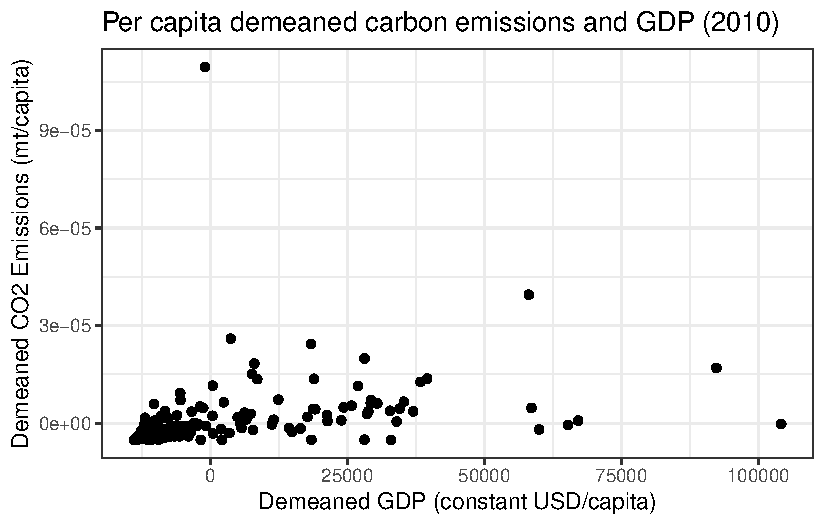
\includegraphics[keepaspectratio]{are212_ps1_files/figure-pdf/unnamed-chunk-10-1.pdf}}

\section{Q11}\label{q11}

\begin{Shaded}
\begin{Highlighting}[]
\NormalTok{wdi\_per\_capita\_log }\OtherTok{\textless{}{-}}
\NormalTok{  wdi\_per\_capita\_demeaned }\SpecialCharTok{\%\textgreater{}\%}
  \FunctionTok{mutate}\NormalTok{(}
    \AttributeTok{CO2pcln =} \FunctionTok{log}\NormalTok{(CO2pc),}
    \AttributeTok{GDPpcln =} \FunctionTok{log}\NormalTok{(GDPpc)}
\NormalTok{  )}
\end{Highlighting}
\end{Shaded}

\section{Q12}\label{q12}

\begin{Shaded}
\begin{Highlighting}[]
\NormalTok{wdi\_per\_capita\_log }\SpecialCharTok{\%\textgreater{}\%}
  \FunctionTok{ggplot}\NormalTok{(}\FunctionTok{aes}\NormalTok{(}\AttributeTok{x =}\NormalTok{ GDPpcln, }\AttributeTok{y =}\NormalTok{ CO2pcln)) }\SpecialCharTok{+}
  \FunctionTok{geom\_point}\NormalTok{() }\SpecialCharTok{+}
  \FunctionTok{scale\_x\_continuous}\NormalTok{(}\StringTok{"Demeaned GDP (constant USD/capita)"}\NormalTok{) }\SpecialCharTok{+}
  \FunctionTok{scale\_y\_continuous}\NormalTok{(}\StringTok{"Demeaned CO2 Emissions (mt/capita)"}\NormalTok{) }\SpecialCharTok{+}
  \FunctionTok{labs}\NormalTok{(}
    \AttributeTok{title =} \StringTok{"Per capita demeaned carbon emissions and GDP (2010)"}
\NormalTok{  ) }\SpecialCharTok{+}
  \FunctionTok{theme\_bw}\NormalTok{()}
\end{Highlighting}
\end{Shaded}

\pandocbounded{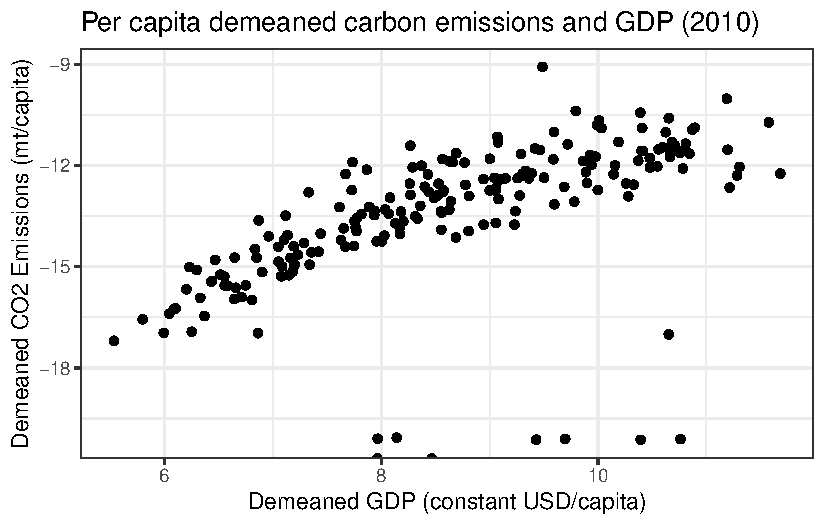
\includegraphics[keepaspectratio]{are212_ps1_files/figure-pdf/unnamed-chunk-12-1.pdf}}

\section{Q13}\label{q13}

\begin{Shaded}
\begin{Highlighting}[]
\NormalTok{  wdi\_per\_capita\_log }\SpecialCharTok{\%\textgreater{}\%}
    \FunctionTok{write\_csv}\NormalTok{(}\AttributeTok{file =} \FunctionTok{file.path}\NormalTok{(path\_data, }\StringTok{"are212\_gold\_ps1\_wdi\_clean.csv"}\NormalTok{))}
\end{Highlighting}
\end{Shaded}

\section{Q14}\label{q14}

We define a custom OLS regression function below

\begin{Shaded}
\begin{Highlighting}[]
\NormalTok{ols }\OtherTok{\textless{}{-}} \ControlFlowTok{function}\NormalTok{(x, y, }\AttributeTok{intercept =} \ConstantTok{FALSE}\NormalTok{) \{}
  
\NormalTok{  X }\OtherTok{\textless{}{-}} \FunctionTok{as.matrix}\NormalTok{(x)}
\NormalTok{  Y }\OtherTok{\textless{}{-}} \FunctionTok{as.matrix}\NormalTok{(y)}

  \ControlFlowTok{if}\NormalTok{(intercept) \{}
\NormalTok{    intercept\_vector }\OtherTok{\textless{}{-}} \FunctionTok{matrix}\NormalTok{(}\DecValTok{1}\NormalTok{, }\FunctionTok{nrow}\NormalTok{(X))}
\NormalTok{    X }\OtherTok{\textless{}{-}} \FunctionTok{cbind}\NormalTok{(intercept\_vector, X)}
\NormalTok{  \}}


\NormalTok{  N }\OtherTok{\textless{}{-}} \FunctionTok{nrow}\NormalTok{(X)}
\NormalTok{  k }\OtherTok{\textless{}{-}} \FunctionTok{ncol}\NormalTok{(X)}
\NormalTok{  b\_ols }\OtherTok{\textless{}{-}} \FunctionTok{solve}\NormalTok{(}\FunctionTok{t}\NormalTok{(X)}\SpecialCharTok{\%*\%}\NormalTok{X) }\SpecialCharTok{\%*\%}\NormalTok{ (}\FunctionTok{t}\NormalTok{(X)}\SpecialCharTok{\%*\%}\NormalTok{Y) }\CommentTok{\# b = (X\textquotesingle{}X)\^{}\{{-}1\}(X\textquotesingle{}Y)}
\NormalTok{  y\_hat }\OtherTok{\textless{}{-}}\NormalTok{ (X) }\SpecialCharTok{\%*\%}\NormalTok{ b\_ols}
  
\NormalTok{  r2\_uc }\OtherTok{\textless{}{-}}\NormalTok{ (}\FunctionTok{t}\NormalTok{(y\_hat)}\SpecialCharTok{\%*\%}\NormalTok{y\_hat) }\SpecialCharTok{/}\NormalTok{ (}\FunctionTok{t}\NormalTok{(Y)}\SpecialCharTok{\%*\%}\NormalTok{Y)}
\NormalTok{  r2 }\OtherTok{\textless{}{-}} \FunctionTok{t}\NormalTok{(y\_hat}\SpecialCharTok{{-}}\FunctionTok{mean}\NormalTok{(Y))}\SpecialCharTok{\%*\%}\NormalTok{(y\_hat}\SpecialCharTok{{-}}\FunctionTok{mean}\NormalTok{(Y)) }\SpecialCharTok{/} \FunctionTok{t}\NormalTok{(Y}\SpecialCharTok{{-}}\FunctionTok{mean}\NormalTok{(Y))}\SpecialCharTok{\%*\%}\NormalTok{(Y}\SpecialCharTok{{-}}\FunctionTok{mean}\NormalTok{(Y))}
\NormalTok{  r2 }\OtherTok{\textless{}{-}}\NormalTok{ r2[[}\DecValTok{1}\NormalTok{,}\DecValTok{1}\NormalTok{]]}
\NormalTok{  r2\_bar }\OtherTok{\textless{}{-}} \DecValTok{1} \SpecialCharTok{{-}}\NormalTok{ ((N}\DecValTok{{-}1}\NormalTok{)}\SpecialCharTok{/}\NormalTok{(N}\SpecialCharTok{{-}}\NormalTok{k))}\SpecialCharTok{*}\NormalTok{(}\DecValTok{1}\SpecialCharTok{{-}}\NormalTok{r2)}

\NormalTok{  e }\OtherTok{\textless{}{-}}\NormalTok{ Y}\SpecialCharTok{{-}}\NormalTok{y\_hat}
\NormalTok{  s2 }\OtherTok{\textless{}{-}}\NormalTok{ (}\FunctionTok{t}\NormalTok{(e)}\SpecialCharTok{\%*\%}\NormalTok{e)}\SpecialCharTok{/}\NormalTok{(N}\SpecialCharTok{{-}}\NormalTok{k)}

  \FunctionTok{list}\NormalTok{(}
    \AttributeTok{beta =}\NormalTok{ b\_ols,}
    \AttributeTok{X =}\NormalTok{ X,}
    \AttributeTok{Y =}\NormalTok{ Y,}
    \AttributeTok{N =}\NormalTok{ N,}
    \AttributeTok{k =}\NormalTok{ k,}
    \AttributeTok{df =}\NormalTok{ N}\SpecialCharTok{{-}}\NormalTok{k,}
    \AttributeTok{r2\_uc =}\NormalTok{ r2\_uc,}
    \AttributeTok{r2 =}\NormalTok{ r2,}
    \AttributeTok{r2\_bar =}\NormalTok{ r2\_bar,}
    \AttributeTok{y\_hat =}\NormalTok{ y\_hat,}
    \AttributeTok{e =}\NormalTok{ e,}
    \AttributeTok{s2 =}\NormalTok{ s2}
\NormalTok{  )}
\NormalTok{\}}
\end{Highlighting}
\end{Shaded}

Next, run each specification and report OLS coefficients

\begin{Shaded}
\begin{Highlighting}[]
\FunctionTok{ols}\NormalTok{(}
\NormalTok{  wdi\_per\_capita\_log}\SpecialCharTok{$}\NormalTok{GDPpc, }
\NormalTok{  wdi\_per\_capita\_log}\SpecialCharTok{$}\NormalTok{CO2pc}
\NormalTok{)}\SpecialCharTok{$}\NormalTok{beta}
\end{Highlighting}
\end{Shaded}

\begin{verbatim}
             [,1]
[1,] 2.374949e-10
\end{verbatim}

\begin{Shaded}
\begin{Highlighting}[]
\FunctionTok{ols}\NormalTok{(}
\NormalTok{  wdi\_per\_capita\_log}\SpecialCharTok{$}\NormalTok{GDPpc, }
\NormalTok{  wdi\_per\_capita\_log}\SpecialCharTok{$}\NormalTok{CO2pc}\SpecialCharTok{*}\DecValTok{1000}
\NormalTok{)}\SpecialCharTok{$}\NormalTok{beta }\CommentTok{\# the coefficient has been multiplied by 1000)}
\end{Highlighting}
\end{Shaded}

\begin{verbatim}
             [,1]
[1,] 2.374949e-07
\end{verbatim}

\begin{Shaded}
\begin{Highlighting}[]
\NormalTok{ols\_co2\_gdp }\OtherTok{\textless{}{-}} 
  \FunctionTok{ols}\NormalTok{(}
\NormalTok{    wdi\_per\_capita\_log}\SpecialCharTok{$}\NormalTok{GDPpc}\SpecialCharTok{/}\DecValTok{1000}\NormalTok{, }
\NormalTok{    wdi\_per\_capita\_log}\SpecialCharTok{$}\NormalTok{CO2pc}\SpecialCharTok{*}\DecValTok{1000}
\NormalTok{  )}
\NormalTok{ols\_co2\_gdp}\SpecialCharTok{$}\NormalTok{beta}
\end{Highlighting}
\end{Shaded}

\begin{verbatim}
             [,1]
[1,] 0.0002374949
\end{verbatim}

In the last regression, the coefficient is multiplied by a further
factor of 1000

\section{Q15}\label{q15}

\begin{Shaded}
\begin{Highlighting}[]
\DocumentationTok{\#\# N = 197}
\NormalTok{n }\OtherTok{\textless{}{-}} \FunctionTok{nrow}\NormalTok{(wdi\_per\_capita\_log)}

\DocumentationTok{\#\# Degrees of freedom: N{-}k}
\NormalTok{df }\OtherTok{\textless{}{-}}\NormalTok{ n}\DecValTok{{-}1} \CommentTok{\# k=1 because there is no intercept}

\DocumentationTok{\#\# beta}
\NormalTok{b }\OtherTok{\textless{}{-}}\NormalTok{ ols\_co2\_gdp}\SpecialCharTok{$}\NormalTok{beta}

\DocumentationTok{\#\# R\^{}2 uncentered}
\NormalTok{ols\_co2\_gdp}\SpecialCharTok{$}\NormalTok{r2\_uc}
\end{Highlighting}
\end{Shaded}

\begin{verbatim}
          [,1]
[1,] 0.2636317
\end{verbatim}

\begin{Shaded}
\begin{Highlighting}[]
\DocumentationTok{\#\# R\^{}2}
\NormalTok{ols\_co2\_gdp}\SpecialCharTok{$}\NormalTok{r2}
\end{Highlighting}
\end{Shaded}

\begin{verbatim}
[1] 0.2513099
\end{verbatim}

\begin{Shaded}
\begin{Highlighting}[]
\DocumentationTok{\#\# Adjusted R\^{}2}
\NormalTok{ols\_co2\_gdp}\SpecialCharTok{$}\NormalTok{r2\_bar}
\end{Highlighting}
\end{Shaded}

\begin{verbatim}
[1] 0.2513099
\end{verbatim}

\begin{Shaded}
\begin{Highlighting}[]
\DocumentationTok{\#\# s\^{}2}
\NormalTok{ols\_co2\_gdp}\SpecialCharTok{$}\NormalTok{s2}
\end{Highlighting}
\end{Shaded}

\begin{verbatim}
             [,1]
[1,] 9.410012e-05
\end{verbatim}

\begin{Shaded}
\begin{Highlighting}[]
\NormalTok{predicted\_vs\_actual }\OtherTok{\textless{}{-}}
  \FunctionTok{data.frame}\NormalTok{(}
    \AttributeTok{y\_hat =}\NormalTok{ ols\_co2\_gdp}\SpecialCharTok{$}\NormalTok{y\_hat,}
    \AttributeTok{y =}\NormalTok{ ols\_co2\_gdp}\SpecialCharTok{$}\NormalTok{Y}
\NormalTok{)}

\NormalTok{predicted\_vs\_actual }\SpecialCharTok{\%\textgreater{}\%}
  \FunctionTok{ggplot}\NormalTok{(}\FunctionTok{aes}\NormalTok{(}\AttributeTok{x =}\NormalTok{ y, }\AttributeTok{y =}\NormalTok{ y\_hat)) }\SpecialCharTok{+}
  \FunctionTok{geom\_point}\NormalTok{() }\SpecialCharTok{+}
  \FunctionTok{geom\_abline}\NormalTok{() }\SpecialCharTok{+}
  \FunctionTok{coord\_fixed}\NormalTok{() }\SpecialCharTok{+}
  \FunctionTok{scale\_y\_continuous}\NormalTok{(}\AttributeTok{limits =} \FunctionTok{c}\NormalTok{(}\DecValTok{0}\NormalTok{, }\FloatTok{0.03}\NormalTok{)) }\SpecialCharTok{+}
  \FunctionTok{scale\_x\_continuous}\NormalTok{(}\AttributeTok{limits =} \FunctionTok{c}\NormalTok{(}\DecValTok{0}\NormalTok{, }\FloatTok{0.12}\NormalTok{)) }\SpecialCharTok{+}
  \FunctionTok{labs}\NormalTok{(}
    \AttributeTok{title =} \StringTok{"Without intercept"}
\NormalTok{  )}
\end{Highlighting}
\end{Shaded}

\pandocbounded{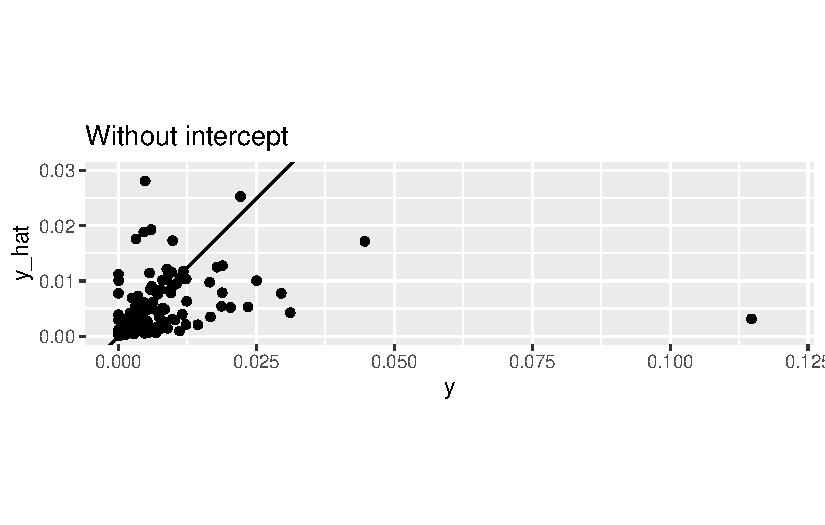
\includegraphics[keepaspectratio]{are212_ps1_files/figure-pdf/unnamed-chunk-16-1.pdf}}

\section{Q16}\label{q16}

\begin{Shaded}
\begin{Highlighting}[]
\NormalTok{ols\_co2\_gdp\_intercept }\OtherTok{\textless{}{-}} 
  \FunctionTok{ols}\NormalTok{(}
\NormalTok{    wdi\_per\_capita\_log}\SpecialCharTok{$}\NormalTok{GDPpc}\SpecialCharTok{/}\DecValTok{1000}\NormalTok{, }
\NormalTok{    wdi\_per\_capita\_log}\SpecialCharTok{$}\NormalTok{CO2pc}\SpecialCharTok{*}\DecValTok{1000}\NormalTok{,}
    \AttributeTok{intercept =} \ConstantTok{TRUE}
\NormalTok{  )}

\DocumentationTok{\#\# beta}
\NormalTok{b\_i }\OtherTok{\textless{}{-}}\NormalTok{ ols\_co2\_gdp\_intercept}\SpecialCharTok{$}\NormalTok{beta}

\DocumentationTok{\#\# R\^{}2 uncentered}
\NormalTok{ols\_co2\_gdp\_intercept}\SpecialCharTok{$}\NormalTok{r2\_uc}
\end{Highlighting}
\end{Shaded}

\begin{verbatim}
          [,1]
[1,] 0.3010531
\end{verbatim}

\begin{Shaded}
\begin{Highlighting}[]
\DocumentationTok{\#\# R\^{}2}
\NormalTok{ols\_co2\_gdp\_intercept}\SpecialCharTok{$}\NormalTok{r2}
\end{Highlighting}
\end{Shaded}

\begin{verbatim}
[1] 0.1173416
\end{verbatim}

\begin{Shaded}
\begin{Highlighting}[]
\DocumentationTok{\#\# Adjusted R\^{}2}
\NormalTok{ols\_co2\_gdp\_intercept}\SpecialCharTok{$}\NormalTok{r2\_bar}
\end{Highlighting}
\end{Shaded}

\begin{verbatim}
[1] 0.1128383
\end{verbatim}

\begin{Shaded}
\begin{Highlighting}[]
\DocumentationTok{\#\# s\^{}2}
\NormalTok{ols\_co2\_gdp\_intercept}\SpecialCharTok{$}\NormalTok{s2}
\end{Highlighting}
\end{Shaded}

\begin{verbatim}
             [,1]
[1,] 8.977376e-05
\end{verbatim}

\begin{Shaded}
\begin{Highlighting}[]
\NormalTok{predicted\_vs\_actual\_intercept }\OtherTok{\textless{}{-}}
  \FunctionTok{data.frame}\NormalTok{(}
    \AttributeTok{y\_hat =}\NormalTok{ ols\_co2\_gdp\_intercept}\SpecialCharTok{$}\NormalTok{y\_hat,}
    \AttributeTok{y =}\NormalTok{ ols\_co2\_gdp\_intercept}\SpecialCharTok{$}\NormalTok{Y,}
    \AttributeTok{x =}\NormalTok{ ols\_co2\_gdp\_intercept}\SpecialCharTok{$}\NormalTok{X[,}\DecValTok{2}\NormalTok{]}
\NormalTok{)}

\NormalTok{predicted\_vs\_actual\_intercept }\SpecialCharTok{\%\textgreater{}\%}
  \FunctionTok{ggplot}\NormalTok{(}\FunctionTok{aes}\NormalTok{(}\AttributeTok{x =}\NormalTok{ y, }\AttributeTok{y =}\NormalTok{ y\_hat)) }\SpecialCharTok{+}
  \FunctionTok{geom\_point}\NormalTok{() }\SpecialCharTok{+}
  \FunctionTok{geom\_abline}\NormalTok{() }\SpecialCharTok{+}
  \FunctionTok{coord\_fixed}\NormalTok{() }\SpecialCharTok{+}
  \FunctionTok{scale\_y\_continuous}\NormalTok{(}\AttributeTok{limits =} \FunctionTok{c}\NormalTok{(}\DecValTok{0}\NormalTok{, }\FloatTok{0.03}\NormalTok{)) }\SpecialCharTok{+}
  \FunctionTok{scale\_x\_continuous}\NormalTok{(}\AttributeTok{limits =} \FunctionTok{c}\NormalTok{(}\DecValTok{0}\NormalTok{, }\FloatTok{0.12}\NormalTok{)) }\SpecialCharTok{+}
  \FunctionTok{labs}\NormalTok{(}
    \AttributeTok{title =} \StringTok{"With intercept"}
\NormalTok{  )}
\end{Highlighting}
\end{Shaded}

\pandocbounded{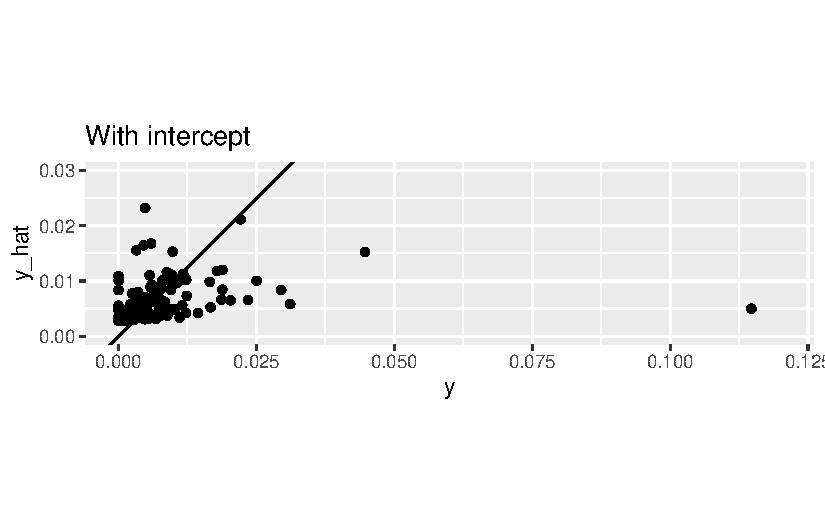
\includegraphics[keepaspectratio]{are212_ps1_files/figure-pdf/unnamed-chunk-17-1.pdf}}

\section{Q17}\label{q17}

\begin{Shaded}
\begin{Highlighting}[]
\NormalTok{wdi\_per\_capita\_quad }\OtherTok{\textless{}{-}}
\NormalTok{  wdi\_per\_capita\_log }\SpecialCharTok{\%\textgreater{}\%}
  \FunctionTok{mutate}\NormalTok{(}
    \AttributeTok{CO2pc\_thou =}\NormalTok{ CO2pc}\SpecialCharTok{*}\DecValTok{1000}\NormalTok{,}
    \AttributeTok{GDPpc\_thou =}\NormalTok{ GDPpc}\SpecialCharTok{/}\DecValTok{1000}\NormalTok{,}
    \AttributeTok{GDPpc\_thou\_2 =}\NormalTok{ (GDPpc\_thou}\SpecialCharTok{\^{}}\DecValTok{2}\NormalTok{)}
\NormalTok{  )}

\NormalTok{ols\_co2\_gdp\_quad }\OtherTok{\textless{}{-}} 
  \FunctionTok{ols}\NormalTok{(}
    \AttributeTok{x =}\NormalTok{ wdi\_per\_capita\_quad }\SpecialCharTok{\%\textgreater{}\%} \FunctionTok{select}\NormalTok{(GDPpc\_thou, GDPpc\_thou\_2),}
    \AttributeTok{y =}\NormalTok{ wdi\_per\_capita\_quad }\SpecialCharTok{\%\textgreater{}\%} \FunctionTok{select}\NormalTok{(CO2pc\_thou),}
    \AttributeTok{intercept =} \ConstantTok{TRUE}
\NormalTok{  )}

\NormalTok{predicted\_vs\_actual\_quad }\OtherTok{\textless{}{-}}
  \FunctionTok{data.frame}\NormalTok{(}
    \AttributeTok{y\_hat =}\NormalTok{ ols\_co2\_gdp\_quad}\SpecialCharTok{$}\NormalTok{y\_hat,}
    \AttributeTok{y =}\NormalTok{ ols\_co2\_gdp\_quad}\SpecialCharTok{$}\NormalTok{Y,}
    \AttributeTok{x =}\NormalTok{ ols\_co2\_gdp\_quad}\SpecialCharTok{$}\NormalTok{X[,}\DecValTok{2}\NormalTok{]}
\NormalTok{) }\SpecialCharTok{\%\textgreater{}\%}
  \FunctionTok{rename}\NormalTok{(}\AttributeTok{y\_hat =} \DecValTok{1}\NormalTok{, }\AttributeTok{y =} \DecValTok{2}\NormalTok{, }\AttributeTok{x =} \DecValTok{3}\NormalTok{)}

\NormalTok{predicted\_vs\_actual\_quad }\SpecialCharTok{\%\textgreater{}\%}
  \FunctionTok{ggplot}\NormalTok{(}\FunctionTok{aes}\NormalTok{(}\AttributeTok{x =}\NormalTok{ y, }\AttributeTok{y =}\NormalTok{ y\_hat)) }\SpecialCharTok{+}
  \FunctionTok{geom\_point}\NormalTok{() }\SpecialCharTok{+}
  \FunctionTok{geom\_abline}\NormalTok{() }\SpecialCharTok{+}
  \FunctionTok{coord\_fixed}\NormalTok{() }\SpecialCharTok{+}
  \FunctionTok{scale\_y\_continuous}\NormalTok{(}\AttributeTok{limits =} \FunctionTok{c}\NormalTok{(}\DecValTok{0}\NormalTok{, }\FloatTok{0.03}\NormalTok{)) }\SpecialCharTok{+}
  \FunctionTok{scale\_x\_continuous}\NormalTok{(}\AttributeTok{limits =} \FunctionTok{c}\NormalTok{(}\DecValTok{0}\NormalTok{, }\FloatTok{0.12}\NormalTok{)) }\SpecialCharTok{+}
  \FunctionTok{labs}\NormalTok{(}
    \AttributeTok{title =} \StringTok{"With intercept + quadratic term"}
\NormalTok{  )}
\end{Highlighting}
\end{Shaded}

\pandocbounded{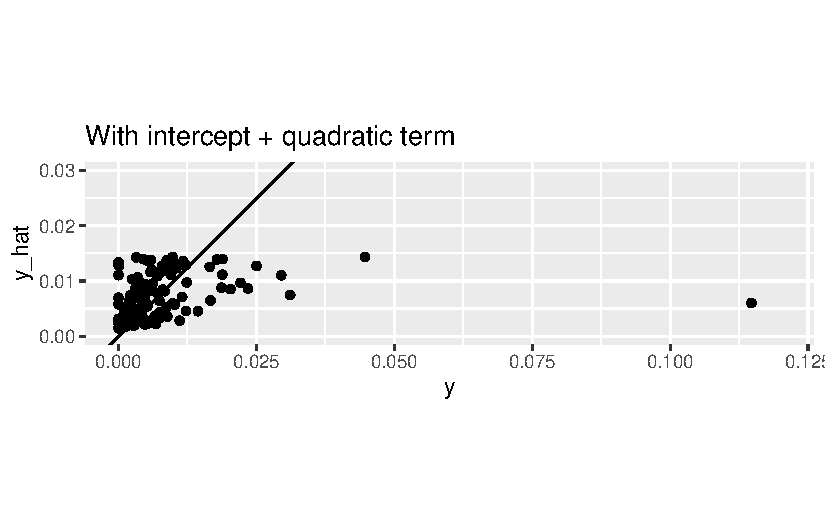
\includegraphics[keepaspectratio]{are212_ps1_files/figure-pdf/unnamed-chunk-18-1.pdf}}

In this regression, we now add a quadratic term for GDP per capita. This
does not violate the first two assumptions. We are still linear in
parameters; it's just that we're linear in a squared term now too. We
still have full rank because the quadratic term is not a simple
rescaling of our original GDP per capita term.

We may have violated spherical errors, though it's hard to tell for
sure.

The specification does make economic sense. This is the Kuznets Curve
story, where firms adopt industrize as they develop but then develop
cleaner technology once they get rich enough.

\section{Q18}\label{q18}

\begin{Shaded}
\begin{Highlighting}[]
\NormalTok{wdi\_per\_capita\_demean }\OtherTok{\textless{}{-}}
\NormalTok{  wdi\_per\_capita\_quad }\SpecialCharTok{\%\textgreater{}\%}
  \FunctionTok{mutate}\NormalTok{(}
    \AttributeTok{CO2pc\_thou\_demean =}\NormalTok{ CO2pc\_thou }\SpecialCharTok{{-}} \FunctionTok{mean}\NormalTok{(CO2pc\_thou),}
    \AttributeTok{GDPpc\_thou\_demean =}\NormalTok{ GDPpc\_thou }\SpecialCharTok{{-}} \FunctionTok{mean}\NormalTok{(GDPpc\_thou),}
    \AttributeTok{GDPpc\_thou\_2\_demean =}\NormalTok{ GDPpc\_thou\_2 }\SpecialCharTok{{-}} \FunctionTok{mean}\NormalTok{(GDPpc\_thou\_2)}
\NormalTok{  )}

\NormalTok{ols\_co2\_gdp\_demean }\OtherTok{\textless{}{-}}
  \FunctionTok{ols}\NormalTok{(}
    \AttributeTok{x =}\NormalTok{ wdi\_per\_capita\_demean }\SpecialCharTok{\%\textgreater{}\%} \FunctionTok{select}\NormalTok{(GDPpc\_thou\_demean, GDPpc\_thou\_2\_demean),}
    \AttributeTok{y =}\NormalTok{ wdi\_per\_capita\_demean }\SpecialCharTok{\%\textgreater{}\%} \FunctionTok{select}\NormalTok{(CO2pc\_thou\_demean),}
    \AttributeTok{intercept =} \ConstantTok{FALSE}
\NormalTok{  )}
  
\NormalTok{ols\_co2\_gdp\_quad}\SpecialCharTok{$}\NormalTok{beta}
\end{Highlighting}
\end{Shaded}

\begin{verbatim}
                CO2pc_thou
              1.295359e-03
GDPpc_thou    3.959382e-04
GDPpc_thou_2 -2.979636e-06
\end{verbatim}

\begin{Shaded}
\begin{Highlighting}[]
\NormalTok{ols\_co2\_gdp\_demean}\SpecialCharTok{$}\NormalTok{beta}
\end{Highlighting}
\end{Shaded}

\begin{verbatim}
                    CO2pc_thou_demean
GDPpc_thou_demean        3.959382e-04
GDPpc_thou_2_demean     -2.979636e-06
\end{verbatim}

The beta's we get from a regression where we demean the variables will
be about the same to the results we get from question 17. Even though we
do not include an explicit intercept, the demeaning allows us to recover
the results from question 17 because we are centering the data at zero
and keeping the slope the same.

\section{Q19}\label{q19}

\begin{Shaded}
\begin{Highlighting}[]
\NormalTok{ols\_co2\_gdp\_q19 }\OtherTok{\textless{}{-}} 
  \FunctionTok{ols}\NormalTok{(}
    \AttributeTok{x =}\NormalTok{ wdi\_per\_capita\_quad }\SpecialCharTok{\%\textgreater{}\%} \FunctionTok{select}\NormalTok{(GDPpc\_thou),}
    \AttributeTok{y =}\NormalTok{ wdi\_per\_capita\_quad }\SpecialCharTok{\%\textgreater{}\%} \FunctionTok{select}\NormalTok{(CO2pc\_thou),}
    \AttributeTok{intercept =} \ConstantTok{TRUE}
\NormalTok{  )}

\NormalTok{resid\_q19 }\OtherTok{\textless{}{-}}\NormalTok{ ols\_co2\_gdp\_q19}\SpecialCharTok{$}\NormalTok{e}

\NormalTok{ols\_1\_gdp }\OtherTok{\textless{}{-}} 
  \FunctionTok{ols}\NormalTok{(}
    \AttributeTok{x =}\NormalTok{ wdi\_per\_capita\_quad }\SpecialCharTok{\%\textgreater{}\%} \FunctionTok{select}\NormalTok{(GDPpc\_thou),}
    \AttributeTok{y =} \FunctionTok{matrix}\NormalTok{(}\DecValTok{1}\NormalTok{, }\AttributeTok{nrow =} \FunctionTok{nrow}\NormalTok{(wdi\_per\_capita\_quad)),}
    \AttributeTok{intercept =} \ConstantTok{FALSE}
\NormalTok{  )}

\NormalTok{ols\_1\_gdp\_resid }\OtherTok{\textless{}{-}}\NormalTok{ ols\_1\_gdp}\SpecialCharTok{$}\NormalTok{e}


\NormalTok{ols\_gdp2\_gdp }\OtherTok{\textless{}{-}} 
  \FunctionTok{ols}\NormalTok{(}
    \AttributeTok{x =}\NormalTok{ wdi\_per\_capita\_quad }\SpecialCharTok{\%\textgreater{}\%} \FunctionTok{select}\NormalTok{(GDPpc\_thou),}
    \AttributeTok{y =}\NormalTok{ wdi\_per\_capita\_quad }\SpecialCharTok{\%\textgreater{}\%} \FunctionTok{select}\NormalTok{(GDPpc\_thou\_2),}
    \AttributeTok{intercept =} \ConstantTok{FALSE}
\NormalTok{  )}

\NormalTok{ols\_gdp2\_gdp\_resid }\OtherTok{\textless{}{-}}\NormalTok{ ols\_gdp2\_gdp}\SpecialCharTok{$}\NormalTok{e}

\NormalTok{resid\_matrix }\OtherTok{\textless{}{-}} \FunctionTok{cbind}\NormalTok{(ols\_1\_gdp\_resid, ols\_gdp2\_gdp\_resid)}

\NormalTok{ols\_resid\_on\_resid }\OtherTok{\textless{}{-}}
  \FunctionTok{ols}\NormalTok{(}
    \AttributeTok{x =}\NormalTok{ resid\_matrix,}
    \AttributeTok{y =}\NormalTok{ resid\_q19,}
    \AttributeTok{intercept =} \ConstantTok{FALSE}
\NormalTok{  )}

\NormalTok{ols\_resid\_on\_resid}\SpecialCharTok{$}\NormalTok{beta}
\end{Highlighting}
\end{Shaded}

\begin{verbatim}
                CO2pc_thou
             -1.387507e-03
GDPpc_thou_2 -2.979636e-06
\end{verbatim}

In question 17, we regressed CO2pc = b1 + b2\emph{GDPpc + b3}GDPpc\^{}2.
In question 19, we regressed CO2pc on GDPpc, and obtained the residual
e1 1 on GDPpc, and obtained the residual e2 GDPpc\^{}2 on GDPpc, and
obtained the residual e3 Finally we regressed e1 = a1\emph{e2 + a2}e3.
we see saw the coefficient on e2 is the same as b1; the coefficient on
e3 is the same as b3. That is, a1 = b1 and a2 = b3. This is an another
example of FWL Thereom in action. Removing the variation in the CO2pc,
1, and GDPpc\^{}2 that comes from GDPpc and using the residual variation
as regressand/regressors gives you the same coefficients as the original
equation in Q17.




\end{document}
